\documentclass{beamer}
\usepackage[utf8]{inputenc}

\usetheme{Madrid}
\usecolortheme{default}
\usepackage{amsmath,amssymb,amsfonts,amsthm}
\usepackage{txfonts}
\usepackage{tkz-euclide}
\usepackage{listings}
\usepackage{adjustbox}
\usepackage{array}
\usepackage{tabularx}
\usepackage{gvv}
\usepackage{lmodern}
\usepackage{circuitikz}
\usepackage{tikz}
\usepackage{graphicx}

\setbeamertemplate{page number in head/foot}[totalframenumber]

\usepackage{tcolorbox}
\tcbuselibrary{minted,breakable,xparse,skins}



\definecolor{bg}{gray}{0.95}
\DeclareTCBListing{mintedbox}{O{}m!O{}}{%
  breakable=true,
  listing engine=minted,
  listing only,
  minted language=#2,
  minted style=default,
  minted options={%
    linenos,
    gobble=0,
    breaklines=true,
    breakafter=,,
    fontsize=\small,
    numbersep=8pt,
    #1},
  boxsep=0pt,
  left skip=0pt,
  right skip=0pt,
  left=25pt,
  right=0pt,
  top=3pt,
  bottom=3pt,
  arc=5pt,
  leftrule=0pt,
  rightrule=0pt,
  bottomrule=2pt,
  toprule=2pt,
  colback=bg,
  colframe=orange!70,
  enhanced,
  overlay={%
    \begin{tcbclipinterior}
    \fill[orange!20!white] (frame.south west) rectangle ([xshift=20pt]frame.north west);
    \end{tcbclipinterior}},
  #3,
}
\lstset{
    language=C,
    basicstyle=\ttfamily\small,
    keywordstyle=\color{blue},
    stringstyle=\color{orange},
    commentstyle=\color{green!60!black},
    numbers=left,
    numberstyle=\tiny\color{gray},
    breaklines=true,
    showstringspaces=false,
}
%------------------------------------------------------------

\title
{5.3.28}
\author 
{AI25BTECH11034 - Sujal Chauhan }



\begin{document}

\frame{\titlepage}
\begin{frame}{Question}


\text{Determine the product}
\myvec
{-4 & 4 & 4 \\
-7 & 1 & 3 \\
5 & -3 & -1}
\myvec{1 & -1 & 1\\
       1 & -2 & -2\\
       2 & 1 & 3}

and use this to solve the equations:

\[
\begin{cases}
x - y + z = 4 \\
x - 2y - 2z = 9 \\
2x + y + 3z = 1
\end{cases}
\]
\end{frame}
\begin{frame}{Solution}

Given equation can be write in form $\Vec{A}\Vec{X}=\Vec{b}$
\begin{align}
    \myvec{1 & -1 & 1\\
       1 & -2 & -2\\
       2 & 1 & 3}\myvec{x \\ y \\z}=\myvec{4\\9\\1}
\end{align}
Let's name our two matrices:
\begin{align}
    \Vec{P} &= \myvec{
        -4 & 4 & 4 \\
        -7 & 1 & 3 \\
        5 & -3 & -1
    } 
    \quad &
    \Vec{Q} &= \myvec{
        1 & -1 & 1 \\
        1 & -2 & -2 \\
        2 & 1 & 3
    }
\end{align}
We can observe that $\Vec{Q}=\Vec{A}$
\end{frame}
\begin{frame}
Now, Let's determine the product $\Vec{P}\Vec{Q}$ of the given two matrices:
\begin{align}
    \myvec
{-4 & 4 & 4 \\
-7 & 1 & 3 \\
5 & -3 & -1}\myvec{1 & -1 & 1\\
       1 & -2 & -2\\
       2 & 1 & 3}=\myvec{
8 & 0 & 0 \\
0 & 8 & 0 \\
0 & 0 & 8
}
\end{align}
\begin{align}
    \Vec{P}\Vec{Q}=8\Vec{I}
\end{align}
Which is multiple of Identity matrix we can use that fact and multiply $\Vec{P}$ both side of our equation.
\begin{align}
    \Vec{P}\Vec{A}\Vec{X}=\Vec{P}\Vec{b}
\end{align}
\begin{align}
    \Vec{X}=\frac{\Vec{P}\Vec{b}}{8}
\end{align}
\end{frame}
\begin{frame}
\begin{align}
    \myvec
{-4 & 4 & 4 \\
-7 & 1 & 3 \\
5 & -3 & -1} \myvec{1 & -1 & 1\\
       1 & -2 & -2\\
       2 & 1 & 3}\myvec{x \\ y \\z}=\myvec
{-4 & 4 & 4 \\
-7 & 1 & 3 \\
5 & -3 & -1}\myvec{4\\9\\1}
\end{align}
\begin{align}
    \myvec{8 & 0 & 0 \\
      0 & 8 & 0 \\
      0 & 0 & 8}
\myvec{x \\ y \\ z}
= 
\myvec{24 \\ -16 \\ -8}
\end{align}
\begin{align}
    \myvec{x \\ y \\ z}
= 
\myvec{3 \\ -2 \\ -1}
\end{align}
\end{frame}
\begin{frame}
\begin{figure}[H]
    \centering
    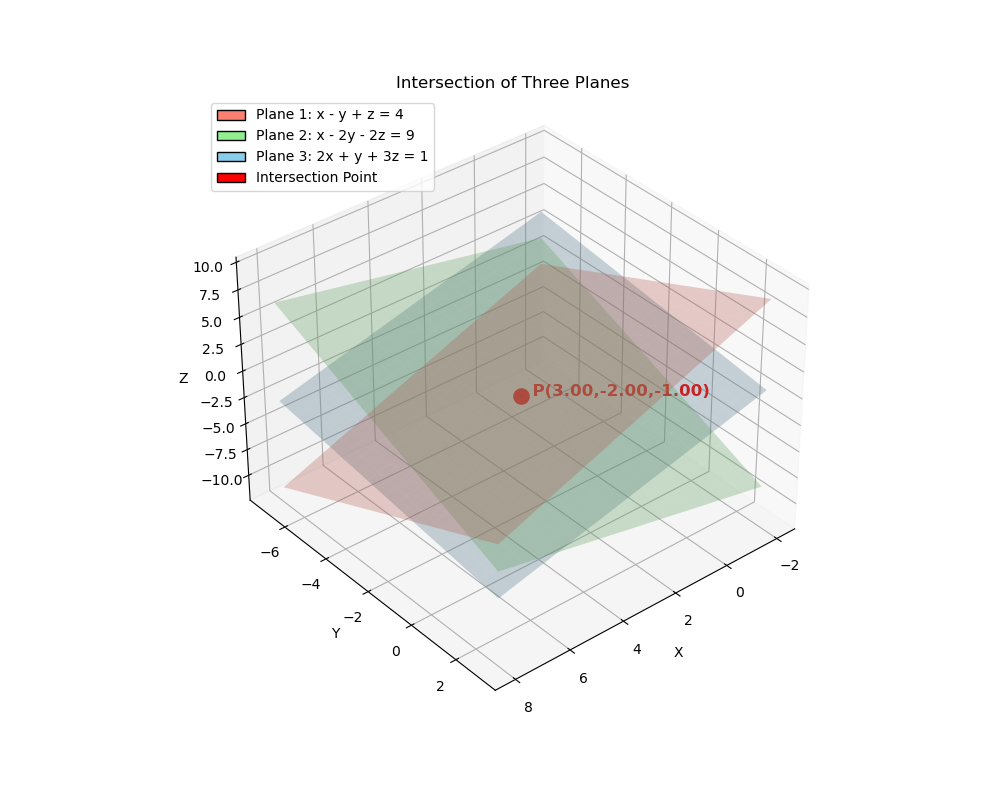
\includegraphics[width=0.5\linewidth]{figures/planes_intersection_c.png}
    \caption{Intersection of three planes}
    \label{fig:placeholder}
\end{figure}




\end{frame}









\end{document}
